\clearpage
\section{Appendices}
  \subsection{Data Dictionary}
    \subsubsection{Actor Descriptions}

    
Identifying actors:\\
\begin{itemize}
  \item Who will supply, use, or remove information from the system?
  \item Who will use the system?
  \item Who is interested in a certain feature or service provided by the system?
  \item Who will support and maintain the system?
  \item What are the system's external resources?
  \item What other systems will need to interact with the system under development?
\end{itemize}

Actors will be the customer/user of the application.  Most interested in our application would be those interested in Bitcoin. Service and maintenance of the system will be performed by the developers(Prestige Worldwide). Systems external resources will be blockchain, SQLite, and other external wallets providing information. (Michael and Brian please confirm external resources of Bitcoin)

    \subsubsection{Use Case Descriptions}
    \begin{figure}[ht]
      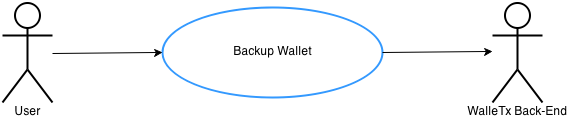
\includegraphics[width=1.0\textwidth]{./chapter7/diagrams/use-case-backup.png}
    \end{figure}

\begin{table}[H]
  \tabulinesep=1.2mm
      \rowcolors{2}{gray!25}{white}
      \begin{tabu}{r | X}
        \rowfont{\color{black}}
        \taburulecolor{white}
        \taburowcolors 2{light-gray .. white}
        \multicolumn{2}{l}{\textbf{\textsf{WalleTx: Backup Data}}}\\
        \hline
        \textsf{Actors} & User\\
        Description & A user will be able to backup all wallet information, transaction hashes, and tags associate with those transactions to an XML or JSON file.\\
        Data & public wallet identification, transaction hashes, tags associate with transactions\\
        Stimulus & User initiates a data backup\\
        Response & Dialog box will confirm backup\\
        Comments & Is there any additional data that needs to be backed up? Where will the database backup be stored?\\
      \end{tabu}
    \end{table}


Identifying use cases:\\
\begin{itemize}
\item What are the goals that the actor will attempt to accomplish with the system?
\item What are the primary tasks that the actor wants the system to perform?
\item Will the actor create, store, change, remove, or read data in the system?
\item Will the actor need to inform the system about sudden external changes?
\item Does the actor need to be informed about certain occurrences, such as unavailability of a network resource, in the system?
\item Will the actor perform a system startup or shutdown?
\end{itemize}

Use cases will be outlined in diagrams provided.\\ 

The primary task of the customer/user will be to interact with the application.  Their main purpose will be to monitor their bitcoin currency from multiple wallets and tag transactions to better organize all transactions.  The actor will have the ability to add and remove wallets/add and remove tags pertaining to transactions. The actor can observe aggregate information in the form of graphs, charts, etc.  The actor will be alerted to certain trigger events. (updated wallet info, specific transactions, etc).  The actor has the ability to close and open application in running OS and also has the ability to completely remove the application from existing OS. \\
	
	
    \subsubsection{Class Descriptions}
      \begin{figure}[H]
        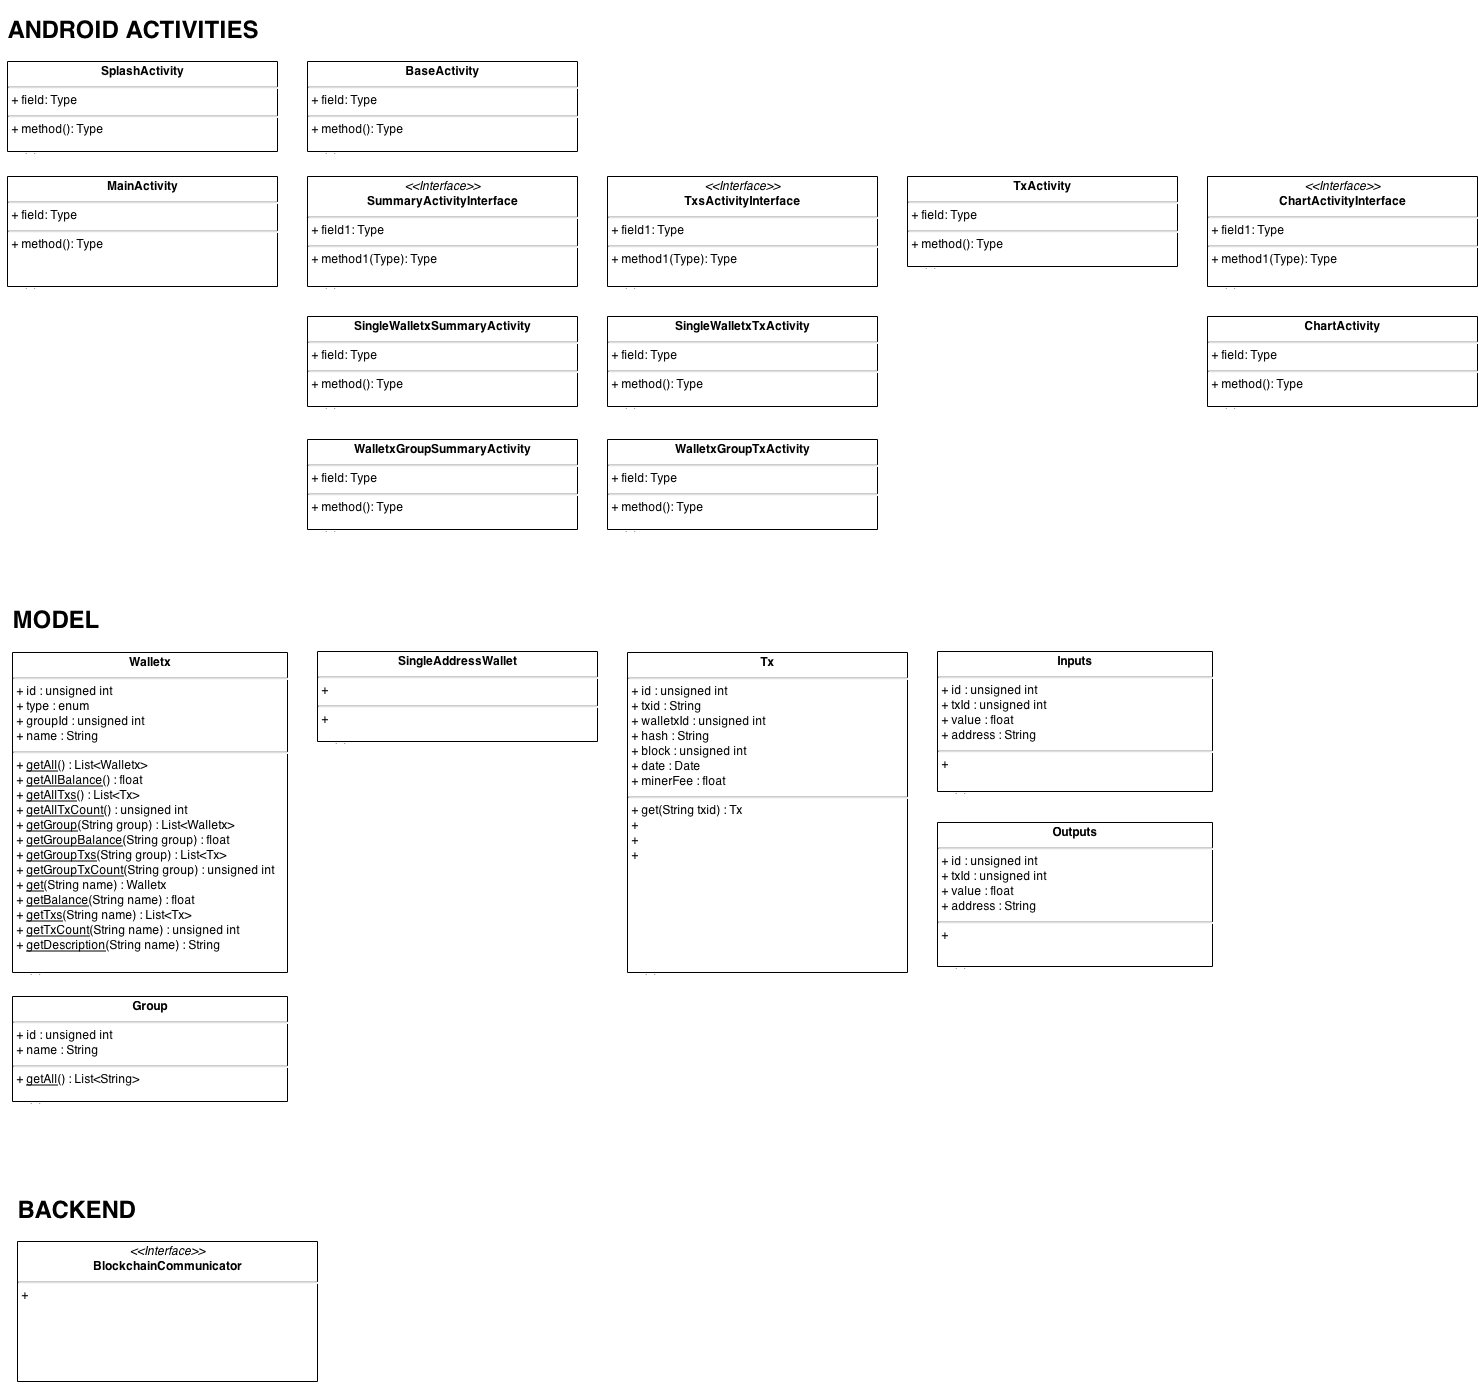
\includegraphics[width=1.0\textwidth]{../diagrams/classes.png}
      \end{figure}

    \subsubsection{Attribute Descriptions}
  \subsection{Raw Use Case Point Analysis}
    \subsubsection{Actor Summary Table}
    \begin{table}[H]
      \begin{tabularx}{\textwidth}{r | X}
        Actors                       & Summary\\
        \hline
        Customer/End User            & This actor will be the end user.  They will interact with WalleTx,  providing it with wallet information, tagging transactions, and viewing  aggrated wallet information\\
        Development Team/Maintenance & This actor will be interacting via the support and maintance of the  application.  They will maintain DB orginzation, revision handling, and  overall maintaince of the application\\
        External Bitcoin Wallets     & External Bitcoin Wallets will be providing our application with vital  information.  All external wallets' totals and transactions will  aggreated in WalleTx.\\
        SQLite Database              & This actor is a database stored on each end user's phone. This will  contain data from wallets, transactions, and display information.  It  will interact soley with the application via code.\\
        Bitcoin Blockchain           & The bitcoin blocktrain will provide transaction specific data for all  included wallets. This actor will interact with the application via  database backend.\\
      \end{tabularx}
    \end{table}

    \subsubsection{Use Case Summary Table}

    \subsubsection{Screens and Reports with Navigation Matrix}
  \subsection{Other Appendices}
